\chapter*{Description du projet}
\addcontentsline{toc}{chapter}{Description du projet}
\label{chap:description}
%\minitoc
L'entreprise Liebherr commercialise des systèmes d'air conditionné qui équipent
la totalité des avions de la gamme A320. Elle assure également la maintenance de ces systèmes sur ces avions. Afin d'être plus compétitive, elle souhaite améliorer son service de maintenance. La firme a constaté que plusieurs de ses clients rencontrent des problèmes et supposent que ceux-ci proviennent de leur manière d'utiliser leurs avions.

Le but de notre projet est d'établir une classification des compagnies aériennes par modes d'opération. Les modes d'opération ont un impact important sur le design des systèmes d'air commercialisés par la société et peuvent expliquer les problèmes rencontrés en service par les compagnies aériennes.

Afin de réaliser cette classification, nous souhaitons exploiter les données de vol ADS-B. L'automatic dependent surveillance-broadcast(ADS-B) est un système de surveillance coopératif pour le contrôle du traffic aérien. Les avions qui utilisent ce système envoient périodiquement leur position, vitesse de montée, vitesse de descente et altitude à des stations positionnées au sol. Les données sont disponibles sur des plateformes open source que l'on peut alors exploiter.

\section*{Objectifs}
\addcontentsline{toc}{section}{Objectifs}
Notre objectif principal sera d'établir une classification des compagnies aériennes par mode d'opération similaire. Cela implique:

\begin{itemize}
	\item extraire des données ADS-B les données de chaque avions de type A320
	\item calculer les phases de vol pour chaque vol
	\item trouver des descripteurs et les calculer pour chaque phase de vol
	\item réaliser une application web pour avoir un aperçu global des données calculées
	\item établir la classification final à partir des données calculées pour chaque vol
\end{itemize}

\section*{Parties prenantes}
\addcontentsline{toc}{section}{Parties prenantes}
Notre client est la société Liebherr avec notamment Nicolas Canouet qui est chargé de l'encadrement du projet. D'un point de vue gestion de projet, Matthieu Bessac se charge de nous accompagner.

\section*{Contraintes associées au projet}
\addcontentsline{toc}{section}{Contraintes associées au projet}
Notre projet se limite à l'étude des données produites par les avions de la gamme A320 puisque notre client ne cherche qu'à établir une classification pour ce type d'avion.

Pour le reste, la forme des rendus par le client est assez libre. Nous prévoyons donc de présenter nos résultats sous forme d'application web accompagnée d'un rapport.

\section*{Exigences}
\addcontentsline{toc}{section}{Exigences}
Les personnes impliquées dans le projet le sont pour une période courte et ne seront plus disponibles une fois le projet terminé. Nous nous devons donc de faire en sorte que nos rendus soient le plus claire possible afin que le client puissent exploiter nos résultats au mieux.

\section*{Synthèse}
\addcontentsline{toc}{section}{Synthèse}
Nous synthétisons dans cette partie le projet par un diagramme pieuvre qui relie les élément externes du système entre eux par l'intermédiaire de celui-ci.

\begin{figure}[!ht]
	\centering
	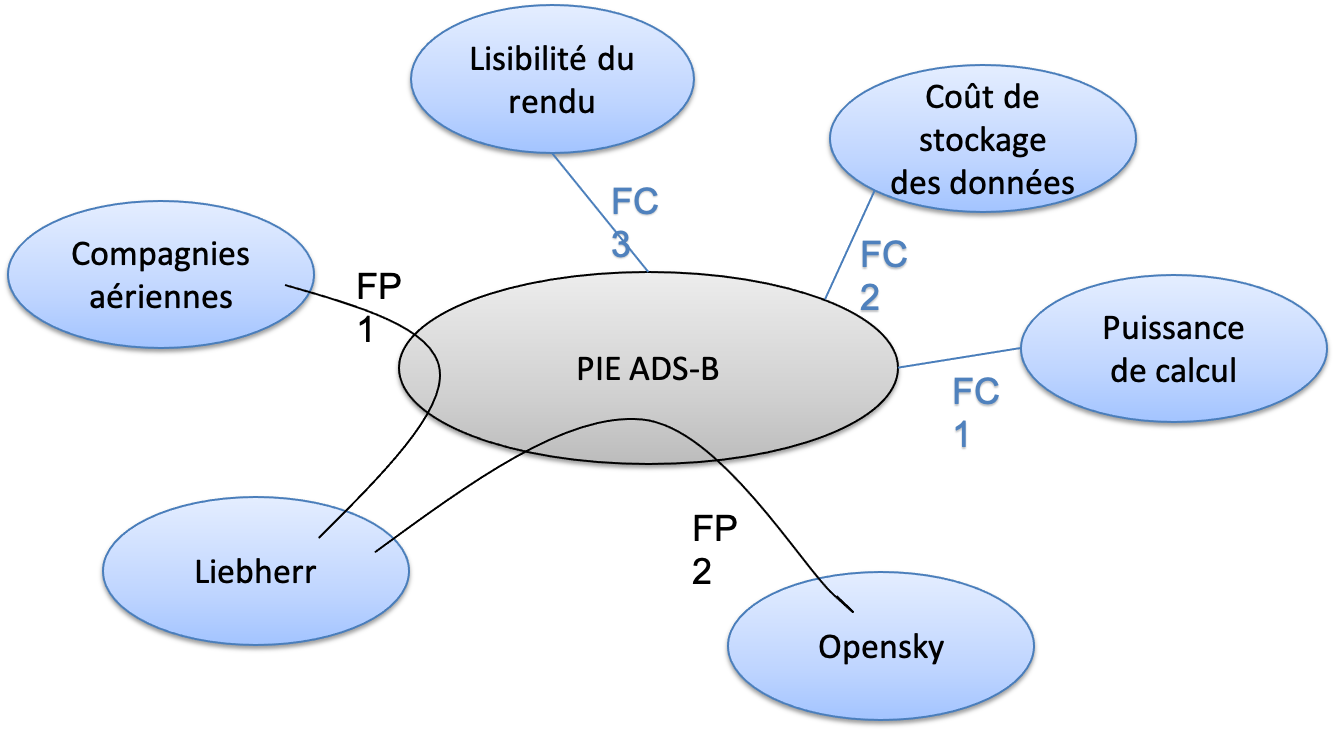
\includegraphics[width=15cm]{DiagrammePieuvre}
	\caption{
		Diagramme pieuvre du projet. FP1: classer les compagnies
		en fonction de leur mode d'opération, FP2: exploiter les données ADS-B
		, FC1: ne pas dépasser les ressources informatiques disponibles,
		FC2: respecter les coûts associés au stockage des données,
		FC3: rendre un projet exploitable par le client.
	}
	\label{fig:pieuvre}
\end{figure}

%%% Local Variables: 
%%% mode: latex
%%% TeX-master: "isae-report-template"
%%% End: 
